
%%%%%%%%%%%%%%%%%%%%%%%%%%%%%%%%%%%%%%%%%%%%%%%%%%%%%%%%%%%%%%%%%%%%%%%%%%%%%%
% Copyright (c) 2003-2018 by The University of Queensland
% http://www.uq.edu.au
%
% Primary Business: Queensland, Australia
% Licensed under the Apache License, version 2.0
% http://www.apache.org/licenses/LICENSE-2.0
%
% Development until 2012 by Earth Systems Science Computational Center (ESSCC)
% Development 2012-2013 by School of Earth Sciences
% Development from 2014 by Centre for Geoscience Computing (GeoComp)
%
%%%%%%%%%%%%%%%%%%%%%%%%%%%%%%%%%%%%%%%%%%%%%%%%%%%%%%%%%%%%%%%%%%%%%%%%%%%%%%

\section{Rayleigh-Taylor Instability}
\label{LEVELSET CHAP}

In this section we will implement the Level Set Method in Escript for tracking the interface between two fluids for Computational Fluid Dynamics (CFD). The method is tested with a Rayleigh-Taylor Instability problem, which is an instability of the interface between two fluids with differing densities. \\ 
Normally in Earth science problems two or more fluids in a system with different properties are of interest. For example, lava dome growth in volcanology, with the contrast of the two mediums as being lava and air. The interface between the two mediums is often referred to as a free surface (free boundary value problem); the problem arises due to the large differences in densities between the lava and air, with their ratio being around 2000, and so the interface between the two fluids move with respect to each other.  
%and so the lava with the much higher density is able to move independently with respect to the air, and the interface between the two fluids is not constrained.
There are a number of numerical techniques to define and track the free surfaces. One of these methods, which is conceptually the simplest, is to construct a Lagrangian grid which moves with the fluid, and so it tracks the free surface. The limitation of this method is that it cannot track surfaces that break apart or intersect. Another limitation is that the elements in the grid can become severely distorted, resulting in numerical instability. The Arbitrary Lagrangian-Eulerian (ALE) method for CFD in moving domains is used to overcome this problem by remeshing, but there is an overhead in computational time, and it results in a loss of accuracy due to the process of mapping the state variables every remesh by interpolation.

There is a technique to overcome these limitations called the Level Set Method, for tracking interfaces between two fluids. The advantages of the method is that CFD can be performed on a fixed Cartesian mesh, and therefore problems with remeshing can be avoided. The field equations for calculating variables such as velocity and pressure are solved on the same mesh. The Level Set Method is based upon the implicit representation of the interface by a continuous function. The function takes the form as a signed distance function, $\phi(x)$, of the interface in a Eulerian coordinate system. For example, the zero isocontour of the unit circle $\phi(x)=x^2 + y^2 -1$ is the set of all points where $\phi(x)=0$. Refer to Figure \ref{UNITCIRCLE}.
%
\begin{figure}
\center
\scalebox{0.8}{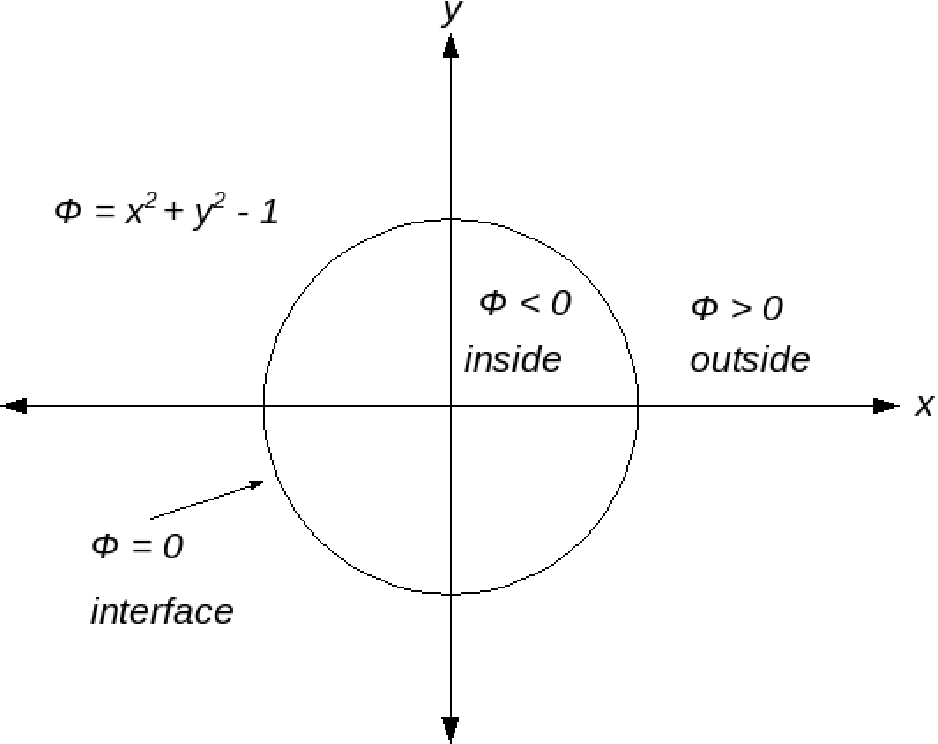
\includegraphics{unitcircle}}
\caption{Implicit representation of the curve $x^2 + y^2 = 1$.}
\label{UNITCIRCLE}
\end{figure}
%
The implicit representation can be used to define the interior and exterior of a fluid region. Since the isocontour at $\phi(x)=0$ has been defined as the interface, a point in the domain can be determined if its inside or outside of the interface, by looking at the local sign of $\phi(x)$. For example, a point is inside the interface when $\phi(x)<0$, and outside the interface when $\phi(x)>0$. Parameters values such as density and viscosity can then be defined for two different mediums, depending on which side of the interface they are located.


\subsection{Calculation of the Displacement of the Interface}

The displacement of the interface at the zero isocontour of $\phi(x)$ is calculated each time-step by using the velocity field. This is achieved my solving the advection equation:
%
\begin{equation}
\frac{\partial \phi}{\partial t} + \vec{v} \cdot \nabla \phi = 0,
\label{ADVECTION}
\end{equation}
%
where $\vec{v}$ is the velocity field. The advection equation is solved using a mid-point, which is a two step procedure:

Firstly, $\phi^{1/2}$ is calculated solving:
%
\begin{equation}
\frac{\phi^{1/2} - \phi^{-}}{dt/2} + \vec{v} \cdot \nabla \phi^{-} = 0.
\label{MIDPOINT FIST}
\end{equation}
%
Secondly, using $\phi^{1/2}$, $\phi^{+}$ is calculated solving:
%
\begin{equation}
\frac{\phi^{+} - \phi^{-}}{dt} + \vec{v} \cdot \nabla \phi^{1/2} = 0.
\label{MIDPOINT SECOND}
\end{equation}
%
This procedure works provided that the discretization of the left-hand side of Equations (\ref{MIDPOINT FIST}) and (\ref{MIDPOINT SECOND}) is a lumped mass matrix. For more details on the mid-point procedure see reference \cite{BOURGOUIN2006}. In certain situations the mid-point procedure has been shown to produce artifacts in the numerical solutions. A more robust procedure is to use the Taylor-Galerkin scheme with the presence of diffusion, which gives more stable solutions. The expression is derived by either inserting Equation (\ref{MIDPOINT FIST}) into Equation (\ref{MIDPOINT SECOND}), or by expanding $\phi$ into a Taylor series:
%
\begin{equation}
\phi^{+} \simeq \phi^{-} + dt\frac{\partial \phi^{-}}{\partial t} + \frac{dt^2}{2}\frac{\partial^{2}\phi^{-}}{\partial t^{2}},
\label{TAYLOR EXPANSION}
\end{equation}
%
by inserting
%
\begin{equation}
\frac{\partial \phi^{-}}{\partial t} = - \vec{v} \cdot \nabla \phi^{-},
\label{INSERT ADVECTION}
\end{equation}
%
and
%
\begin{equation}
\frac{\partial^{2} \phi^{-}}{\partial t^{2}} = \frac{\partial}{\partial t}(-\vec{v} \cdot \nabla \phi^{-}) = \vec{v}\cdot \nabla (\vec{v}\cdot \nabla \phi^{-}),
\label{SECOND ORDER}
\end{equation}
%
into Equation (\ref{TAYLOR EXPANSION})
%
\begin{equation}
\phi^{+} = \phi^{-} - dt\vec{v}\cdot \nabla \phi^{-} + \frac{dt^2}{2}\vec{v}\cdot \nabla (\vec{v}\cdot \nabla \phi^{-}).
\label{TAYLOR GALERKIN}
\end{equation}


%\subsection{Governing Equations for Fluid Flow}

%The fluid dynamics is governed by the Stokes equations. In geophysical problems the velocity of fluids are low; that is, the inertial forces are small compared with the viscous forces, therefore the inertial terms in the Navier-Stokes equations can be ignored. For a body force $f$ the governing equations are given by:
%
%\begin{equation}
%\nabla \cdot (\eta(\nabla \vec{v} + \nabla^{T} \vec{v})) - \nabla p = -f,
%\label{GENERAL NAVIER STOKES}
%\end{equation}
%
%with the incompressibility condition
%
%\begin{equation}
%\nabla \cdot \vec{v} = 0.
%\label{INCOMPRESSIBILITY}
%\end{equation}
%
%where $p$, $\eta$ and $f$ are the pressure, viscosity and body forces, respectively. 
%Alternatively, the Stokes equations can be represented in Einstein summation tensor notation (compact notation):
%
%\begin{equation}
%-(\eta(v_{i,j} + v_{j,i})),_{j} - p,_{i} = f_{i},
%\label{GENERAL NAVIER STOKES COM}
%\end{equation}
%
%with the incompressibility condition
%
%\begin{equation}
%-v_{i,i} = 0.
%\label{INCOMPRESSIBILITY COM}
%\end{equation}
%
%The subscript comma $i$ denotes the derivative of the function with respect to $x_{i}$. A linear relationship between the deviatoric stress $\sigma^{'}_{ij}$ and the stretching $D_{ij} = \frac{1}{2}(v_{i,j} + v_{j,i})$ is defined as \cite{GROSS2006}:
%
%\begin{equation}
%\sigma^{'}_{ij} = 2\eta D^{'}_{ij},
%\label{STRESS}
%\end{equation}
%
%where the deviatoric stretching $D^{'}_{ij}$ is defined as
%
%\begin{equation}
%D^{'}_{ij} = D^{'}_{ij} - \frac{1}{3}D_{kk}\delta_{ij}.
%\label{DEVIATORIC STRETCHING}
%\end{equation}
%
%where $\delta_{ij}$ is the Kronecker $\delta$-symbol, which is a matrix with ones for its diagonal entries ($i = j$) and zeros for the remaining entries ($i \neq j$). The body force $f$ in Equation (\ref{GENERAL NAVIER STOKES COM}) is the gravity acting in the $x_{3}$ direction and is given as $f = -g \rho \delta_{i3}$.
%The Stokes equations is a saddle point problem, and can be solved using a Uzawa scheme. A class called StokesProblemCartesian in Escript can be used to solve for velocity and pressure.
%In order to keep numerical stability, the time-step size needs to be below a certain value, known as the Courant number \index{Courant number}\index{CFL condition}. The Courant number is defined as:
%
%\begin{equation}
%C = \frac{v \delta t}{h}.
%\label{COURANT}
%\end{equation}
%
%where $\delta t$, $v$, and $h$ are the time-step, velocity, and the width of an element in the mesh, respectively. The velocity $v$ may be chosen as the maximum velocity in the domain. In this problem the Courant number is taken to be 0.4 \cite{BOURGOUIN2006}.


\subsection{Reinitialization of Interface}

As the computation of the distance function progresses, it becomes distorted, and so it needs to be updated in order to stay regular \cite{SUSSMAN1994}. This process is known as the reinitialization procedure. The aim is to iteratively find a solution to the reinitialization equation:
%
\begin{equation}
\frac{\partial \psi}{\partial \tau} + sign(\phi)(1 - \nabla \psi) = 0.
\label{REINITIALISATION}
\end{equation}
%
where $\psi$ shares the same level set with $\phi$, $\tau$ is pseudo time, and $sign(\phi)$ is the smoothed sign function. This equation is solved to meet the definition of the level set function, $\lvert \nabla \psi \rvert = 1$; the normalization condition. Equation (\ref{REINITIALISATION}) can be rewritten in similar form to the advection equation:
%
\begin{equation}
\frac{\partial \psi}{\partial \tau} + \vec{w} \cdot \nabla \psi = sign(\phi),
\label{REINITIALISATION2}
\end{equation}
%
where
%
\begin{equation}
\vec{w} = sign(\phi)\frac{\nabla \psi}{|\nabla \psi|}.
\label{REINITIALISATION3}
\end{equation}
%
$\vec{w}$ is the characteristic velocity pointing outward from the free surface. Equation (\ref{REINITIALISATION2}) can be solved by a similar technique to what was used in the advection step; either by the mid-point technique \cite{BOURGOUIN2006} or the Taylor-Galerkin procedure. For the mid-point technique, the reinitialization technique algorithm is:

1. Calculate
%
\begin{equation}
\vec{w} = sign(\phi)\frac{\nabla \psi}{|\nabla \psi|},
\label{REINITIAL MIDPOINT1}
\end{equation}
%

2. Calculate $\psi^{1/2}$ solving
%
\begin{equation}
\frac{\psi^{1/2} - \psi^{-}}{d\tau/2} + \vec{w} \cdot \nabla \psi^{-}= sign(\phi),
\label{REINITIAL MIDPOINT2}
\end{equation}
%

3. using $\psi^{1/2}$, calculate $\psi^{+}$ solving
%
\begin{equation}
\frac{\psi^{+} - \psi^{-}}{d\tau} + \vec{w} \cdot \nabla \psi^{1/2}= sign(\phi),
\label{REINITIAL MIDPOINT3}
\end{equation}
%

4. if the convergence criterion has not been met, go back to step 2. Convergence is declared if
%
\begin{equation}
||\nabla \psi _{\infty}| - 1| < \epsilon _{\psi}.
\label{REINITIAL CONVERGE}
\end{equation}
%
where $\epsilon _{\psi}$ is the convergence tolerance. Normally, the reinitialization procedure is performed every third time-step of solving the Stokes equation.

The mid-point technique works provided that the left-hand side of Equations (\ref{REINITIAL MIDPOINT2}) and (\ref{REINITIAL MIDPOINT3}) is a lumped mass matrix. Alternatively, for a one-step procedure, the reinitialization equation can be given by:
%
\begin{equation}
\psi^{+} = \psi^{-} - \tau \vec{w} \cdot \nabla \psi^{-} + \frac{d \tau^{2}}{2} \vec{w} \cdot \nabla(\vec{w} \cdot \nabla \psi^{-}).
\label{REINITIAL ONESTEP}
\end{equation}
%
The accuracy of $\phi$ is only needed within the transition zone; and so it can be calculated in a narrow band between the interface of the fluids. 
%
\begin{figure}
\center
\scalebox{0.5}{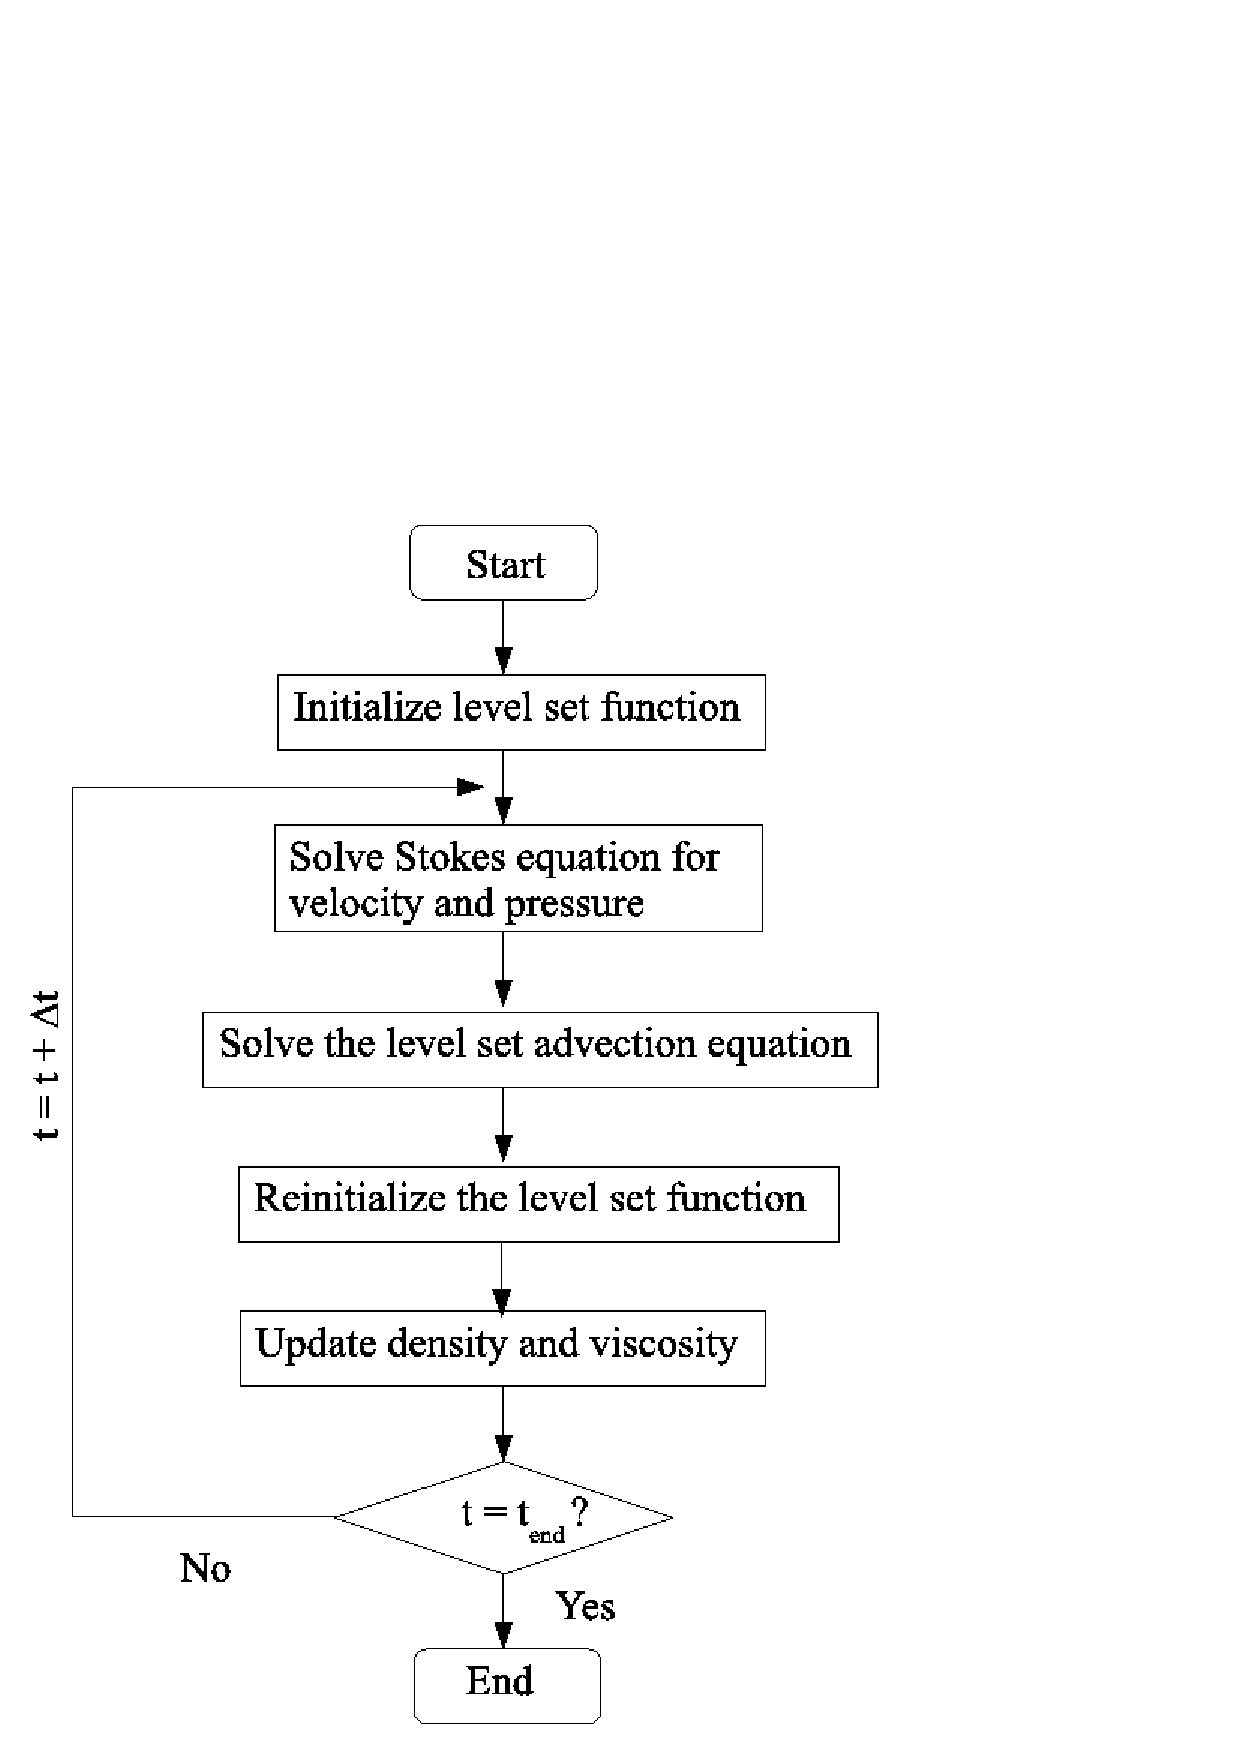
\includegraphics{LevelSetFlowChart}}
\caption{Flow chart of Level Set Method procedure \cite{LIN2005}.}
\label{LEVELSET FLOWCHART}
\end{figure}
%
When the distance function, $\phi$, is calculated, the physical parameters, density and viscosity, are updated using the sign of $\phi$. The jump in material properties between two fluids, such as air and water can be extreme, and so the transition of the properties from one medium to another is smoothed. The region of the interface is assumed to be of finite thickness of $\alpha h$, where $h$ is the size of the elements in the computational mesh and $\alpha$ is a smoothing parameter. The parameters are updated by the following expression:
%
\begin{equation}
P = 
\left \{ \begin{array}{l}
P_{1} \hspace{5cm}  where \ \ \psi < - \alpha h \\
P_{2} \hspace{5cm}  where \ \ \psi > \alpha h \\
(P_{2} - P_{1}) \psi/2\alpha h + (P_{1} + P_{2})/2 \ \ \ \ \ \ where \ \ |\psi| < \alpha h.
\end{array}
\right.
\label{UPDATE PARAMETERS}
\end{equation} 
%
where the subscripts $1$ and $2$ denote the different fluids. The procedure of the level set calculation is shown in Figure \ref{LEVELSET FLOWCHART}.
Further work is needed in the reinitialization procedure, as it has been shown that it is prone to mass loss and inconsistent positioning of the interface \cite{SUCKALE2008}.

\subsection{Benchmark Problem}

The Rayleigh-Taylor instability problem is used as a benchmark to validate CFD implementations \cite{VANKEKEN1997}. Figure \ref{RT2DSETUP} shows the setup of the problem. A rectangular domain with two different fluids is considered, with the greater density fluid on the top and the lighter density fluid on the bottom. The viscosities of the two fluids are equal (isoviscous). An initial perturbation is given to the interface of $\phi=0.02cos(\frac{\pi x}{\lambda}) + 0.2$. The aspect ratio $\lambda = L/H = 0.9142$ is chosen such that it gives the greatest disturbance of the fluids. The fluid properties is chosen such that the compositional Rayleigh number is equal to one:
%
\begin{equation}
R_{b} = \frac{\Delta \rho H^{3}}{\kappa \eta} = 1.
\label{RAYLEIGH NUMBER}
\end{equation}
%
where $\Delta \rho$ is the difference in density between the two fluids, $\eta$ is the viscosity and $\kappa$ is the thermal diffusivity; arbitrarily taken equal to 1 for a ``non thermal'' case.
%
%
\begin{figure}
\center
\scalebox{0.7}{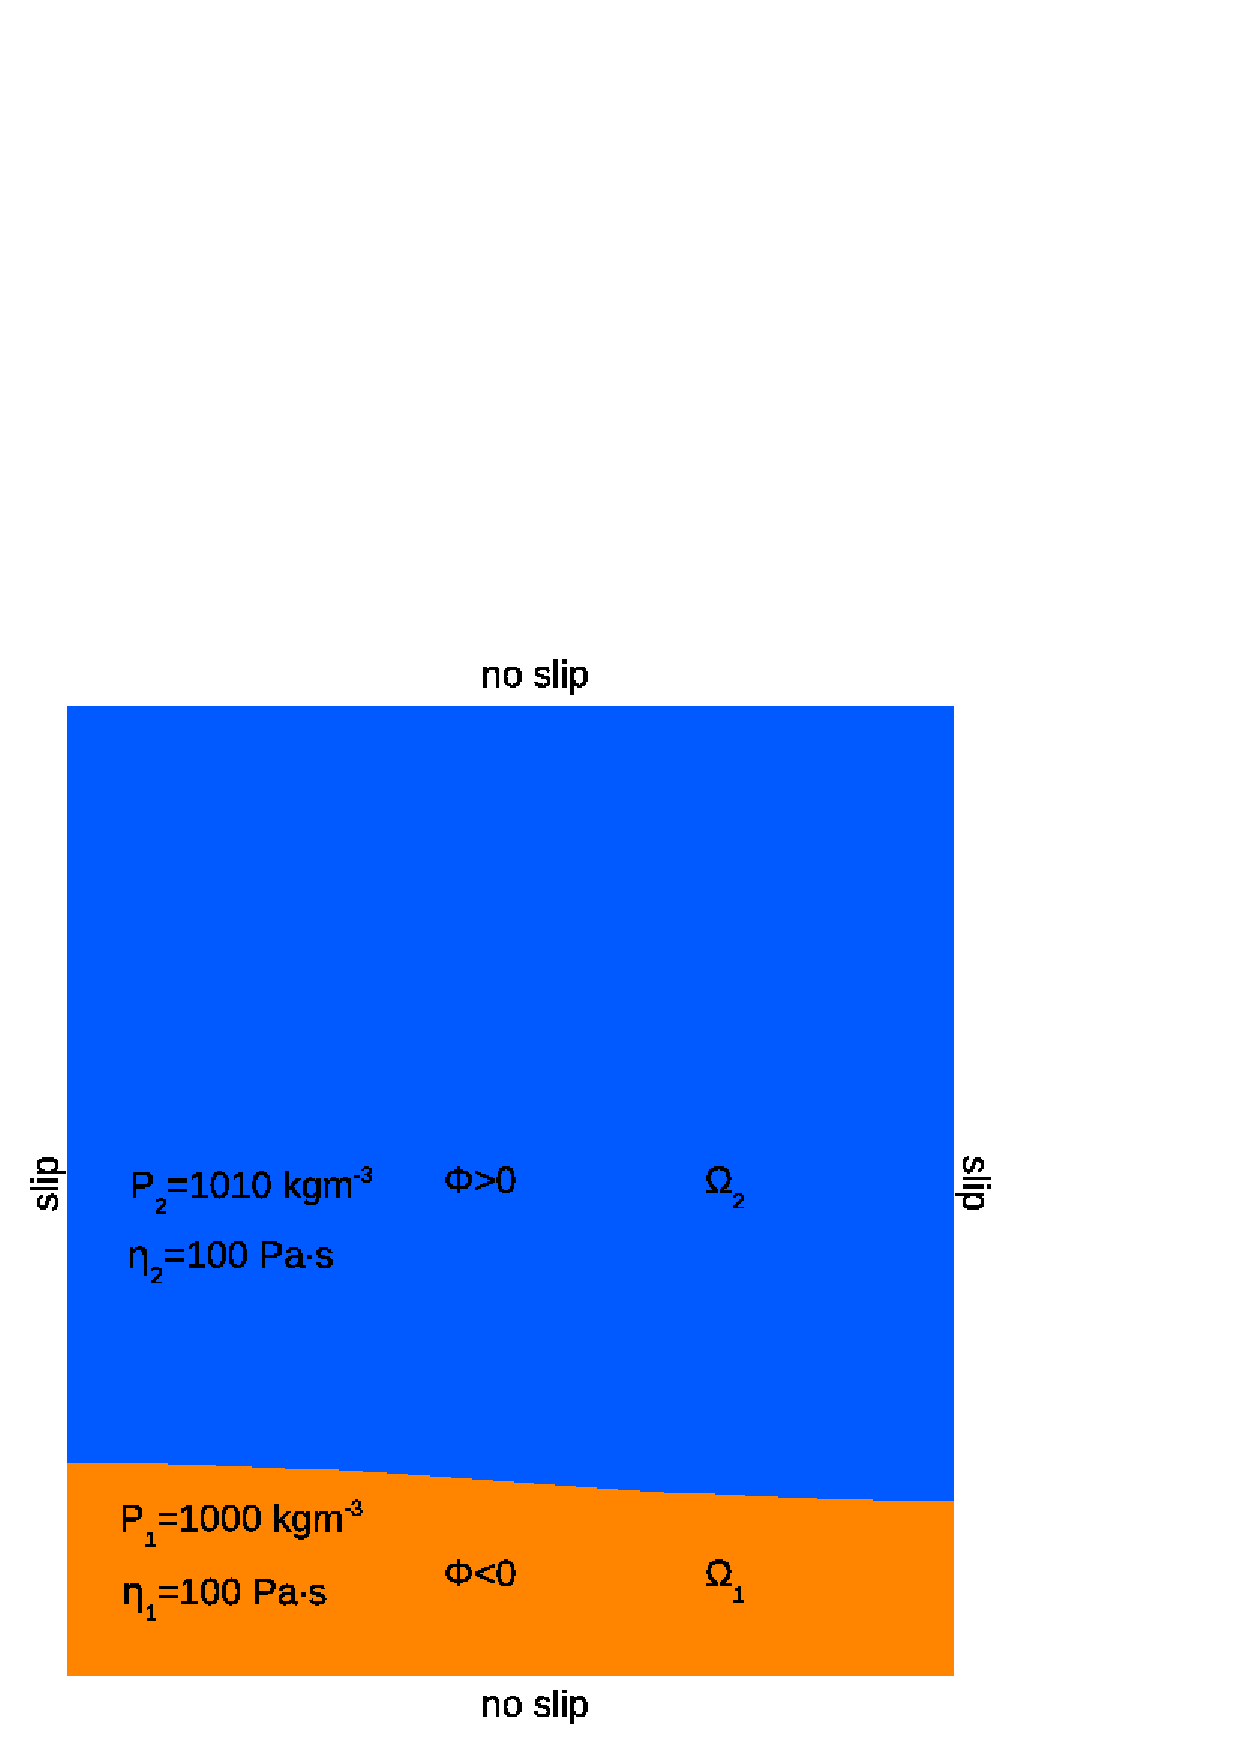
\includegraphics{RT2Dsetup}}
\caption{Parameters, initial interface and boundary conditions for the Rayleigh-Taylor instability problem. The interface is defined as $\phi=0.02cos(\frac{\pi x}{\lambda}) + 0.2$. The fluids have been assigned different densities and equal viscosity (isoviscous) \cite{BOURGOUIN2006}.}
\label{RT2DSETUP}
\end{figure}
%
%
The following PYTHON code is for the Rayleigh-Taylor instability problem, which is available in the example directory as 'RT2D.py'. This script uses the 'StokesProblemCartesian' class for solving the Stokes equation, along with the incompressibility condition. A class called 'LevelSet' is also used, which performs the advection and reinitialization procedures to track the movement of the interface of the fluids. The details and use of these classes are described in Chapter \ref{MODELS CHAPTER} (Models Chapter).

The script starts off by importing the necessary classes. The physical properties of the two fluids are defined, such as density and viscosity.
Acceleration due to gravity is taken as 10.0 $ms^{-2}$.
Solver settings are set for solving the Stokes problem, with the number of time-steps, solver tolerance, maximum solver iterations,
and the option to use the Uzawa scheme or not; the default solver is the PCG solver. A regular mesh is defined with 200$\times$200 elements. 
Level set parameters are set for the reinitialization procedure, such as the convergence tolerance, number of 
reinitialization steps, the frequency of the reinitialization, for example, every third time-step, and the smoothing
 parameter to smooth the physical properties across the interface.
 A no-slip boundary condition is set for the top and bottom of the domain, while on the left and right-hand sides
 there is a slip condition. 
The initial interface between the two fluids is defined as in Figure \ref{RT2DSETUP}. Instances of the StokesProblemCartesian and LevelSet class are created. 
The iteration throughout the time-steps involves the update of the physical parameters of the fluids; the initialization of 
the boundary conditions, viscosity, and body forces; the solving of the Stokes problem for velocity and pressure; then the 
level set procedure. 
The output of the level set function, velocity and pressure is saved to file. 
The time-step size is selected based on the Courant-Friedrichs-Lewy condition (CFL condition)\index{Courant number}\index{CFL condition}. 
Due to the number of elements in the computational mesh, the simulation may take a long time to complete on a desktop computer, 
so it is preferable to run it on the super computer. 
At present, the fine mesh is required to capture the details of the fluid motion and for numerical stability.  
%
\begin{python}

from esys.escript import *
import esys.finley
from esys.escript.models import StokesProblemCartesian
from esys.finley import finley
from esys.finley import Rectangle
from esys.weipa import saveVTK
from LevelSet import *

#physical properties
rho1 = 1000		#fluid density on bottom
rho2 = 1010		#fluid density on top
eta1 = 100.0		#fluid viscosity on bottom
eta2 = 100.0		#fluid viscosity on top
g=10.0

#solver settings
dt = 0.001
t_step = 0
t_step_end = 2000
TOL = 1.0e-5
max_iter=400
verbose=True
useUzawa=True

#define mesh
l0=0.9142
l1=1.0
n0=200      
n1=200

mesh=Rectangle(l0=l0, l1=l1, order=2, n0=n0, n1=n1)
#get mesh dimensions
numDim = mesh.getDim()
#get element size
h = Lsup(mesh.getSize())

#level set parameters
tolerance = 1.0e-6
reinit_max = 30
reinit_each = 3
alpha = 1
smooth = alpha*h 

#boundary conditions
x = mesh.getX()
#left + bottom + right + top
b_c = whereZero(x[0])*[1.0,0.0] + whereZero(x[1])*[1.0,1.0] + whereZero(x[0]-l0)*[1.0,0.0] \
      + whereZero(x[1]-l1)*[1.0,1.0]

velocity = Vector(0.0, ContinuousFunction(mesh))
pressure = Scalar(0.0, ContinuousFunction(mesh))
Y = Vector(0.0,Function(mesh))

#define initial interface between fluids
xx = mesh.getX()[0]
yy = mesh.getX()[1]
func = Scalar(0.0, ContinuousFunction(mesh))
h_interface = Scalar(0.0, ContinuousFunction(mesh))
h_interface = h_interface + (0.02*cos(math.pi*xx/l0) + 0.2)
func = yy - h_interface
func_new = func.interpolate(ReducedSolution(mesh))

#Stokes Cartesian
solution=StokesProblemCartesian(mesh,debug=True)
solution.setTolerance(TOL)
solution.setSubProblemTolerance(TOL**2)

#level set
levelset = LevelSet(mesh, func_new, reinit_max, reinit_each, tolerance, smooth)    

while t_step <= t_step_end:
  #update density and viscosity
  rho = levelset.update_parameter(rho1, rho2)
  eta = levelset.update_parameter(eta1, eta2)

  #get velocity and pressure of fluid
  Y[1] = -rho*g
  solution.initialize(fixed_u_mask=b_c,eta=eta,f=Y)
  velocity,pressure=solution.solve(velocity,pressure,max_iter=max_iter,verbose=verbose, \ 
  useUzawa=useUzawa)
  
  #update the interface
  func = levelset.update_phi(velocity, dt, t_step)  

  print("##########################################################")
  print("time step:", t_step, " completed with dt:", dt)
  print("Velocity: min =", inf(velocity), "max =", Lsup(velocity))
  print("##########################################################")
 
  #save interface, velocity and pressure 
  saveVTK("phi2D.%2.4i.vtu"%t_step,interface=func,velocity=velocity,pressure=pressure)
  #CFL condition
  dt = 0.4*Lsup(mesh.getSize())/Lsup(velocity)
  t_step += 1

\end{python}
%
%
The results from the simulation can be viewed by visualization software such as \textit{visIt}. If the software is installed, it can be opened by simply executing the following command:
%
\begin{python}
visit
\end{python}
%
In the visIt main window, vtk/vtu files can be opened from the File menu; contours and vectors can then be displayed by selecting them from the Plots menu and pressing the Draw button. A movie of the simulation can be watched by pressing the Play button. The graphics are displayed in the Vis window. For more information on \textit{visIt} see the website \cite{VisIt}.

The simulation output is shown in Figures \ref{RT2D OUTPUT1} and \ref{RT2D OUTPUT1} showing the progression of the interface of the two fluids. A diapir can be seen rising on the left-hand side of the domain, and then later on, a second one rises on the right-hand side.
\begin{figure}
\center
\subfigure[t=300]{\label{RT OUTPUT300}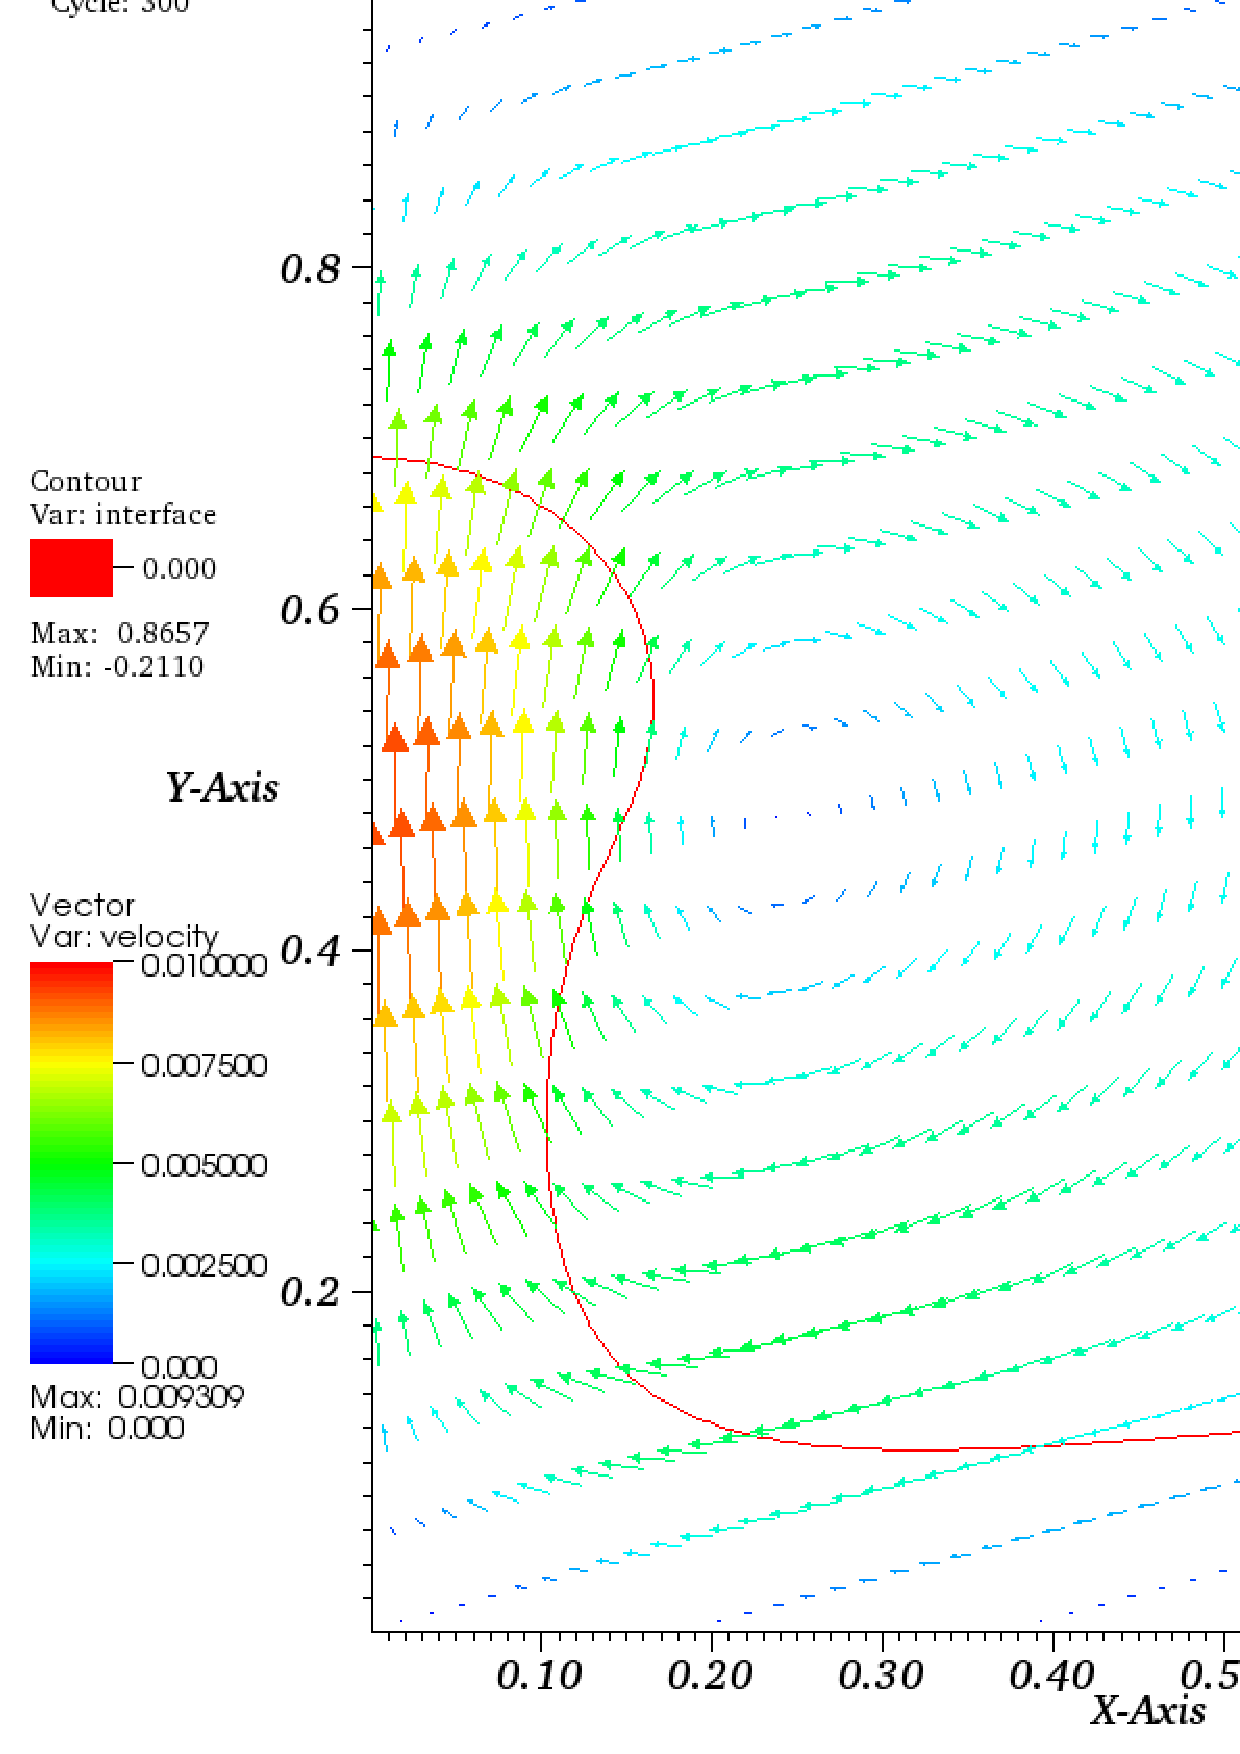
\includegraphics[scale=0.252]{RT2D200by200t300}}
\subfigure[t=600]{\label{RT OUTPUT600}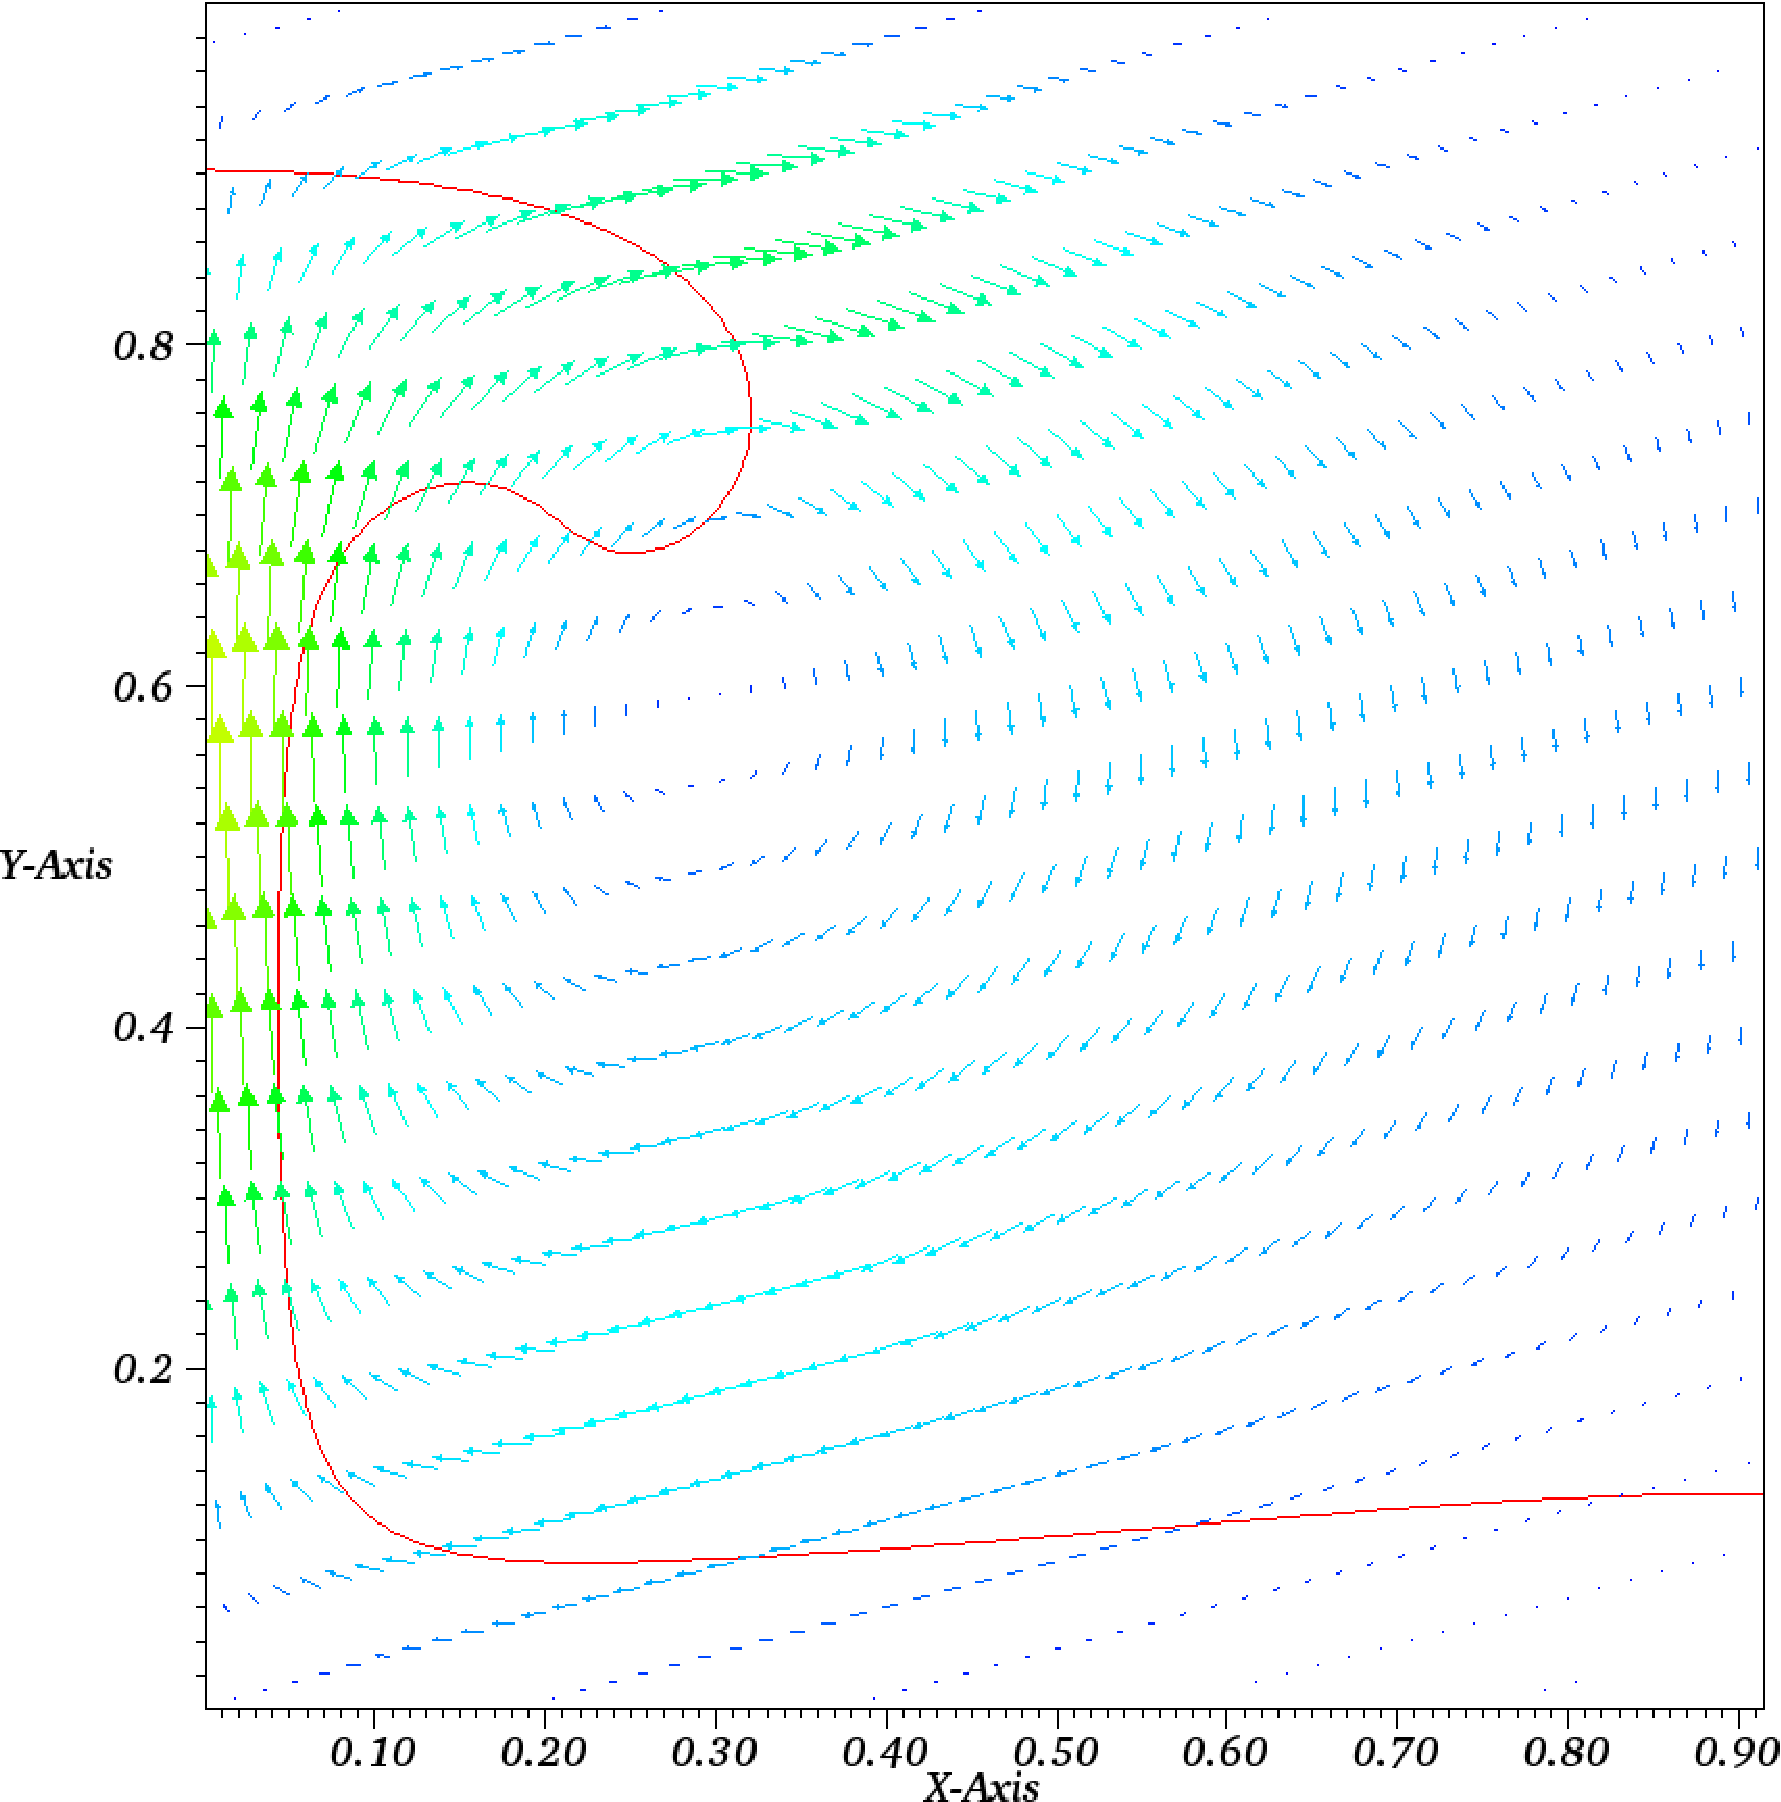
\includegraphics[scale=0.252]{RT2D200by200t600}}
\subfigure[t=900]{\label{RT OUTPUT900}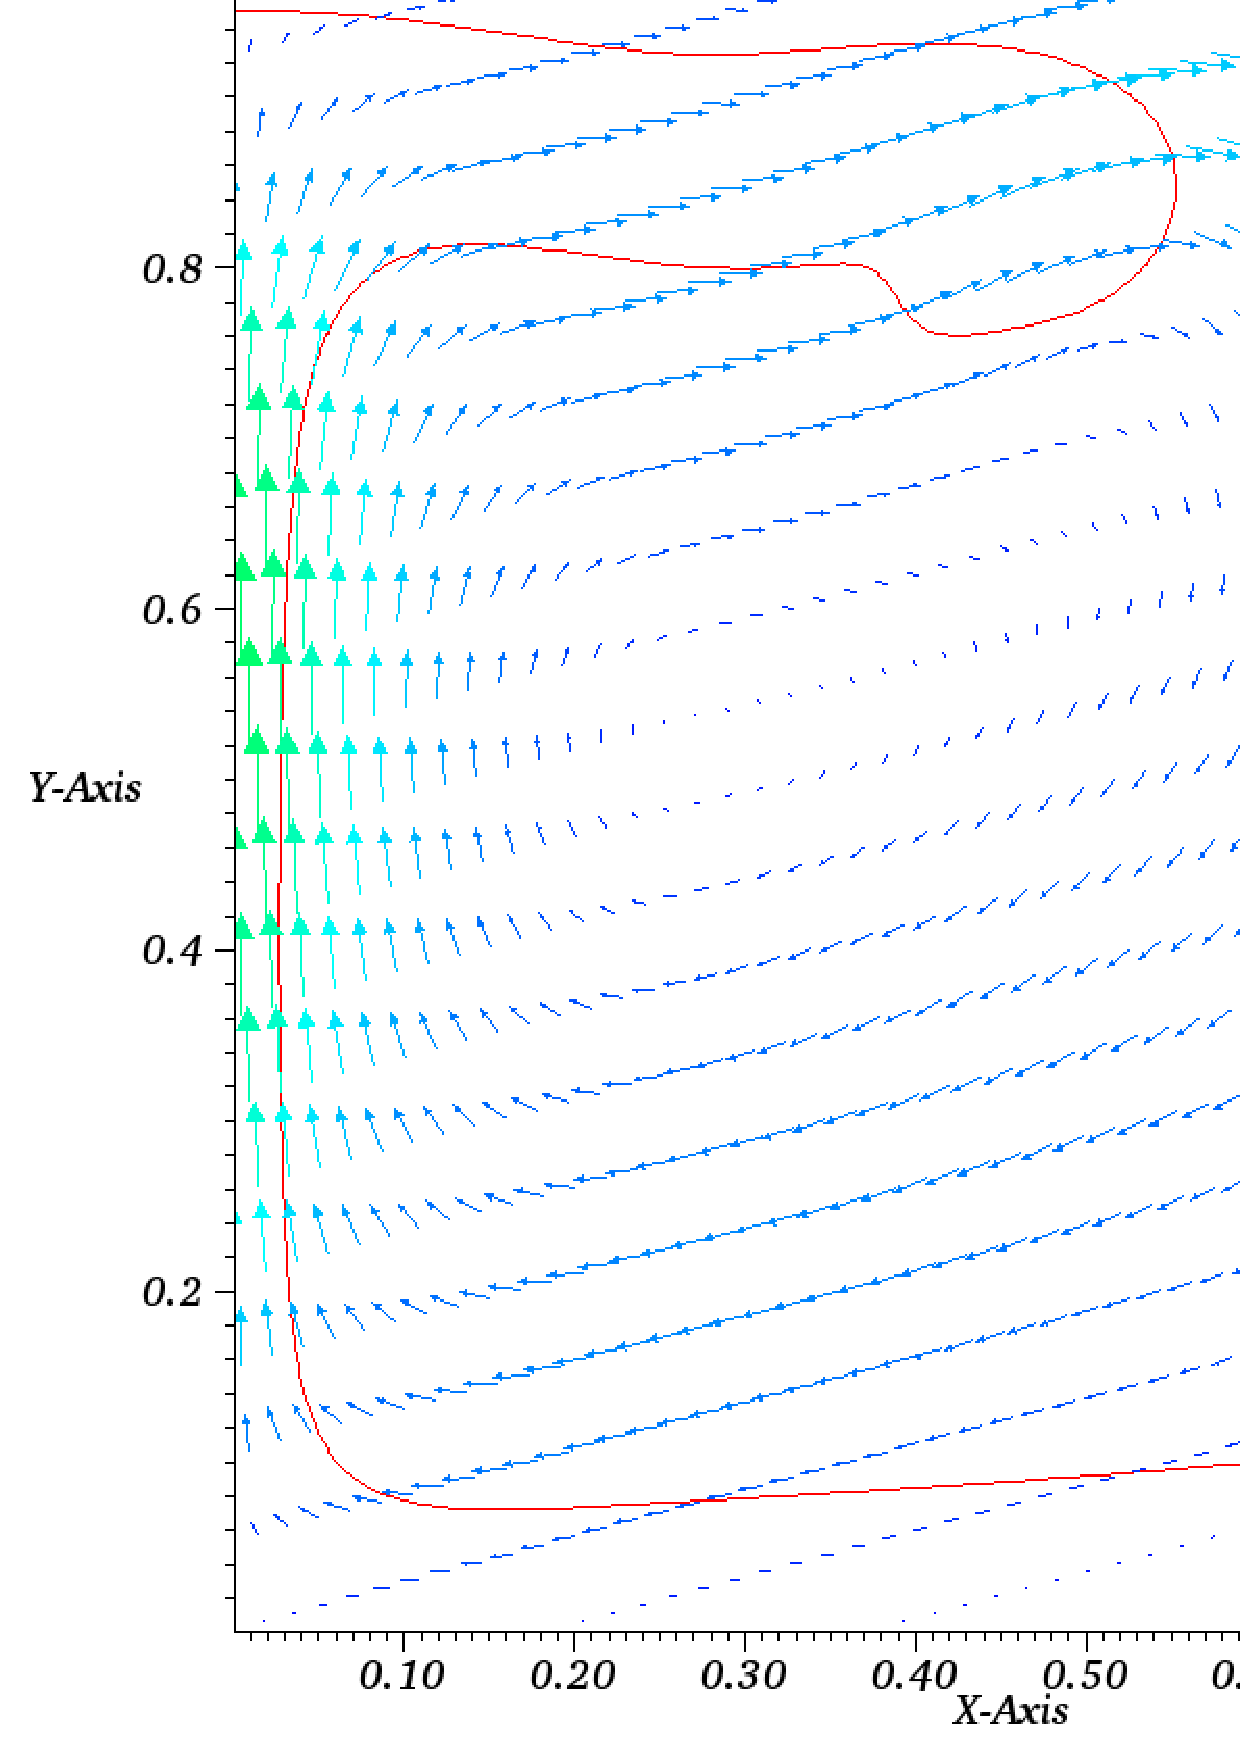
\includegraphics[scale=0.252]{RT2D200by200t900}}
\subfigure[t=1200]{\label{RT OUTPUT1200}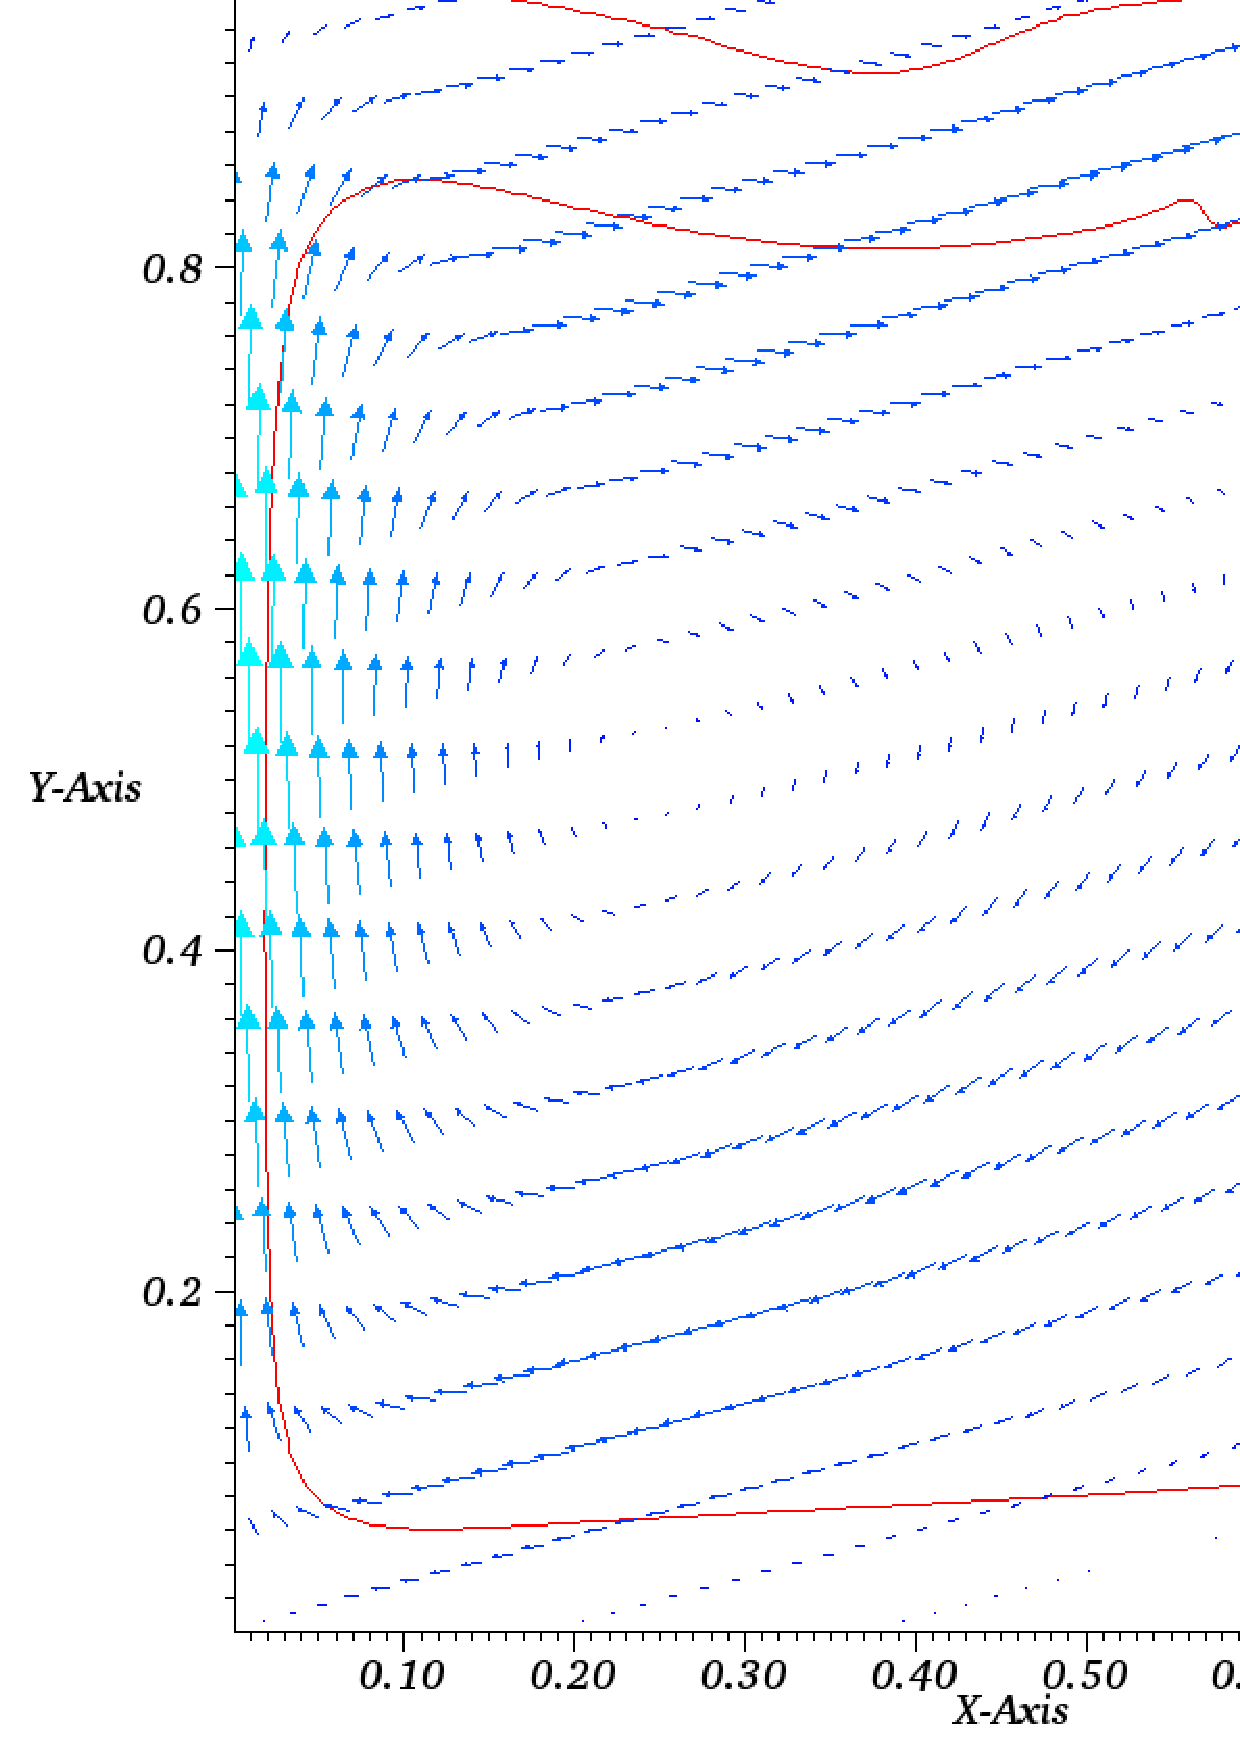
\includegraphics[scale=0.252]{RT2D200by200t1200}}
\caption{Simulation output of Rayleigh-Taylor instability, showing the movement of the interface of the fluids. The contour line represents the interface between the two fluids; the zero contour of the Level Set function. Velocity vectors are displayed showing the flow field. Computational mesh used was 200$\times$200 elements.}
\label{RT2D OUTPUT1}
\end{figure}
%
\begin{figure}
\center
\subfigure[t=1500]{\label{RT OUTPUT1500}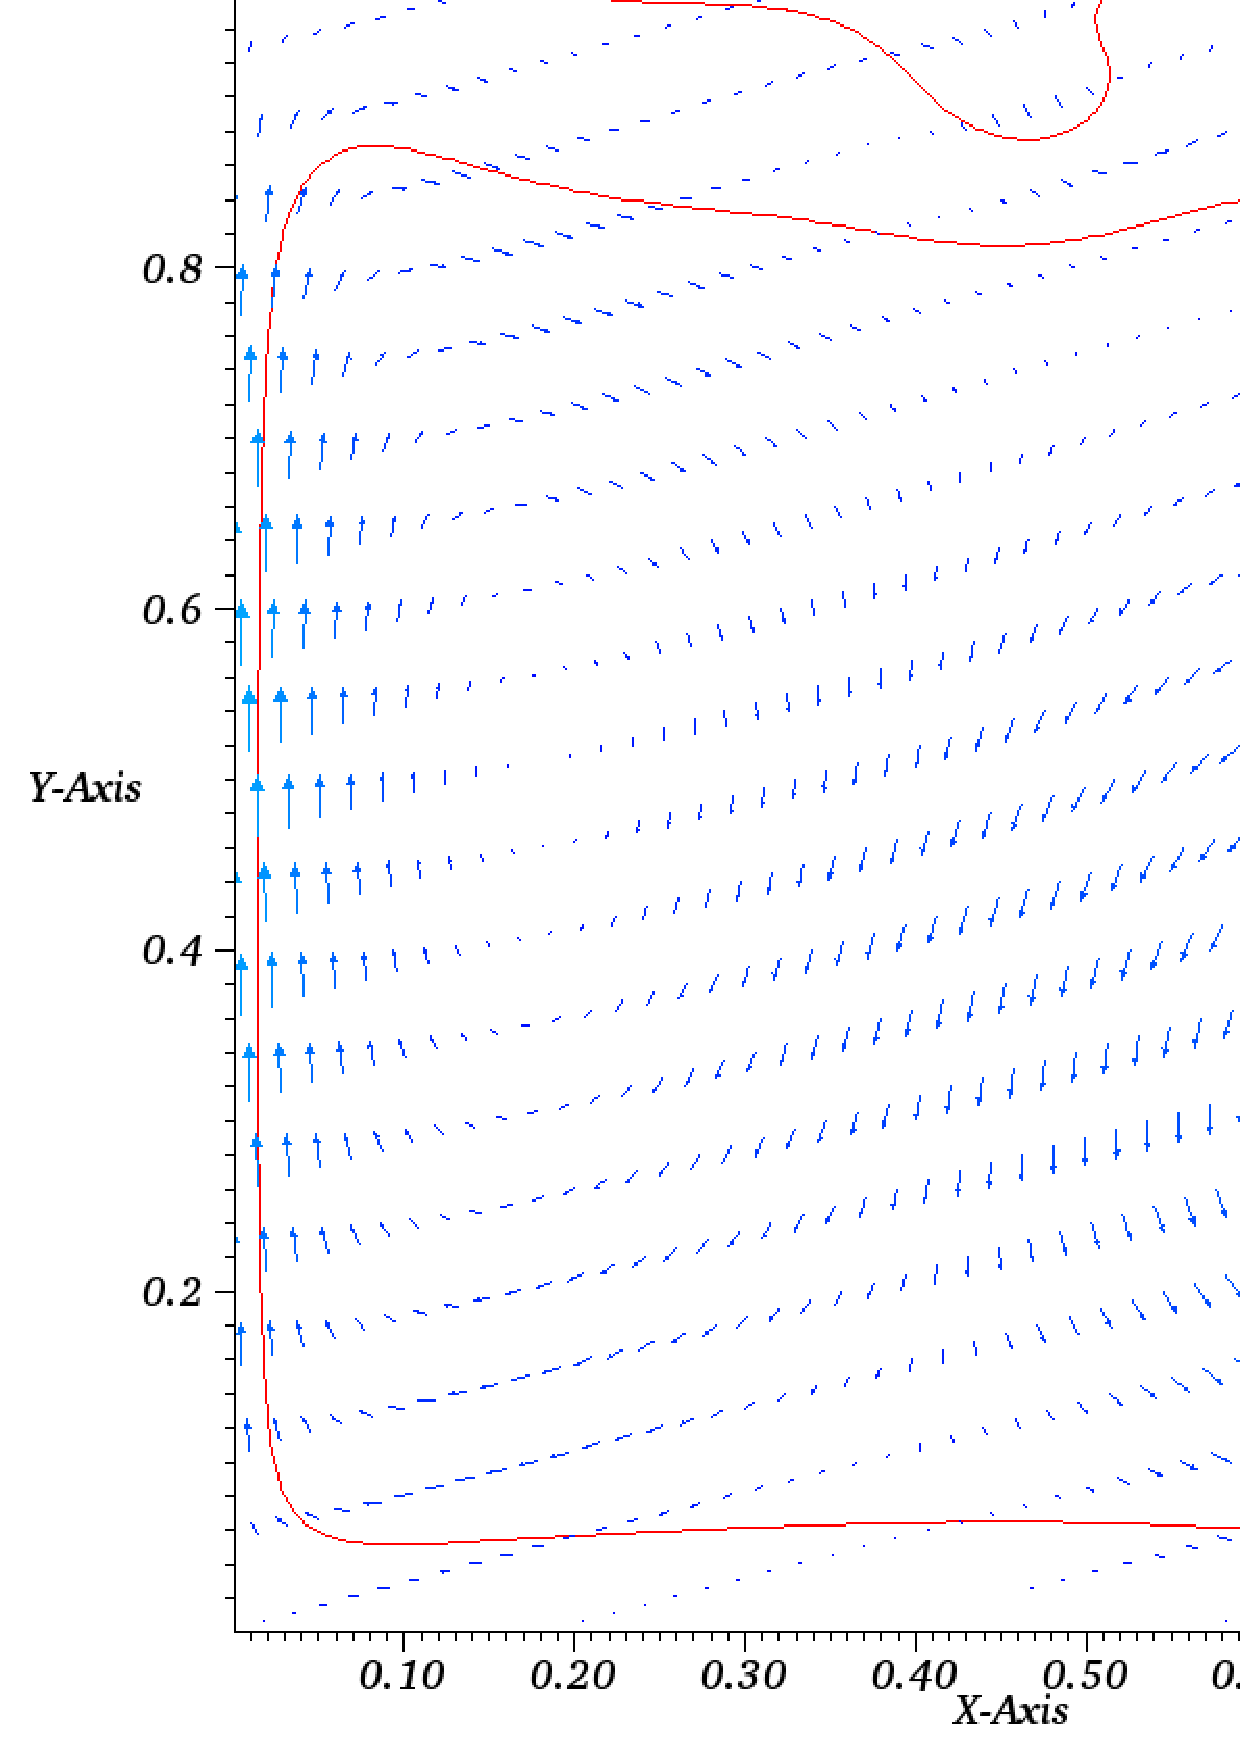
\includegraphics[scale=0.252]{RT2D200by200t1500}}
\subfigure[t=1800]{\label{RT OUTPUT1800}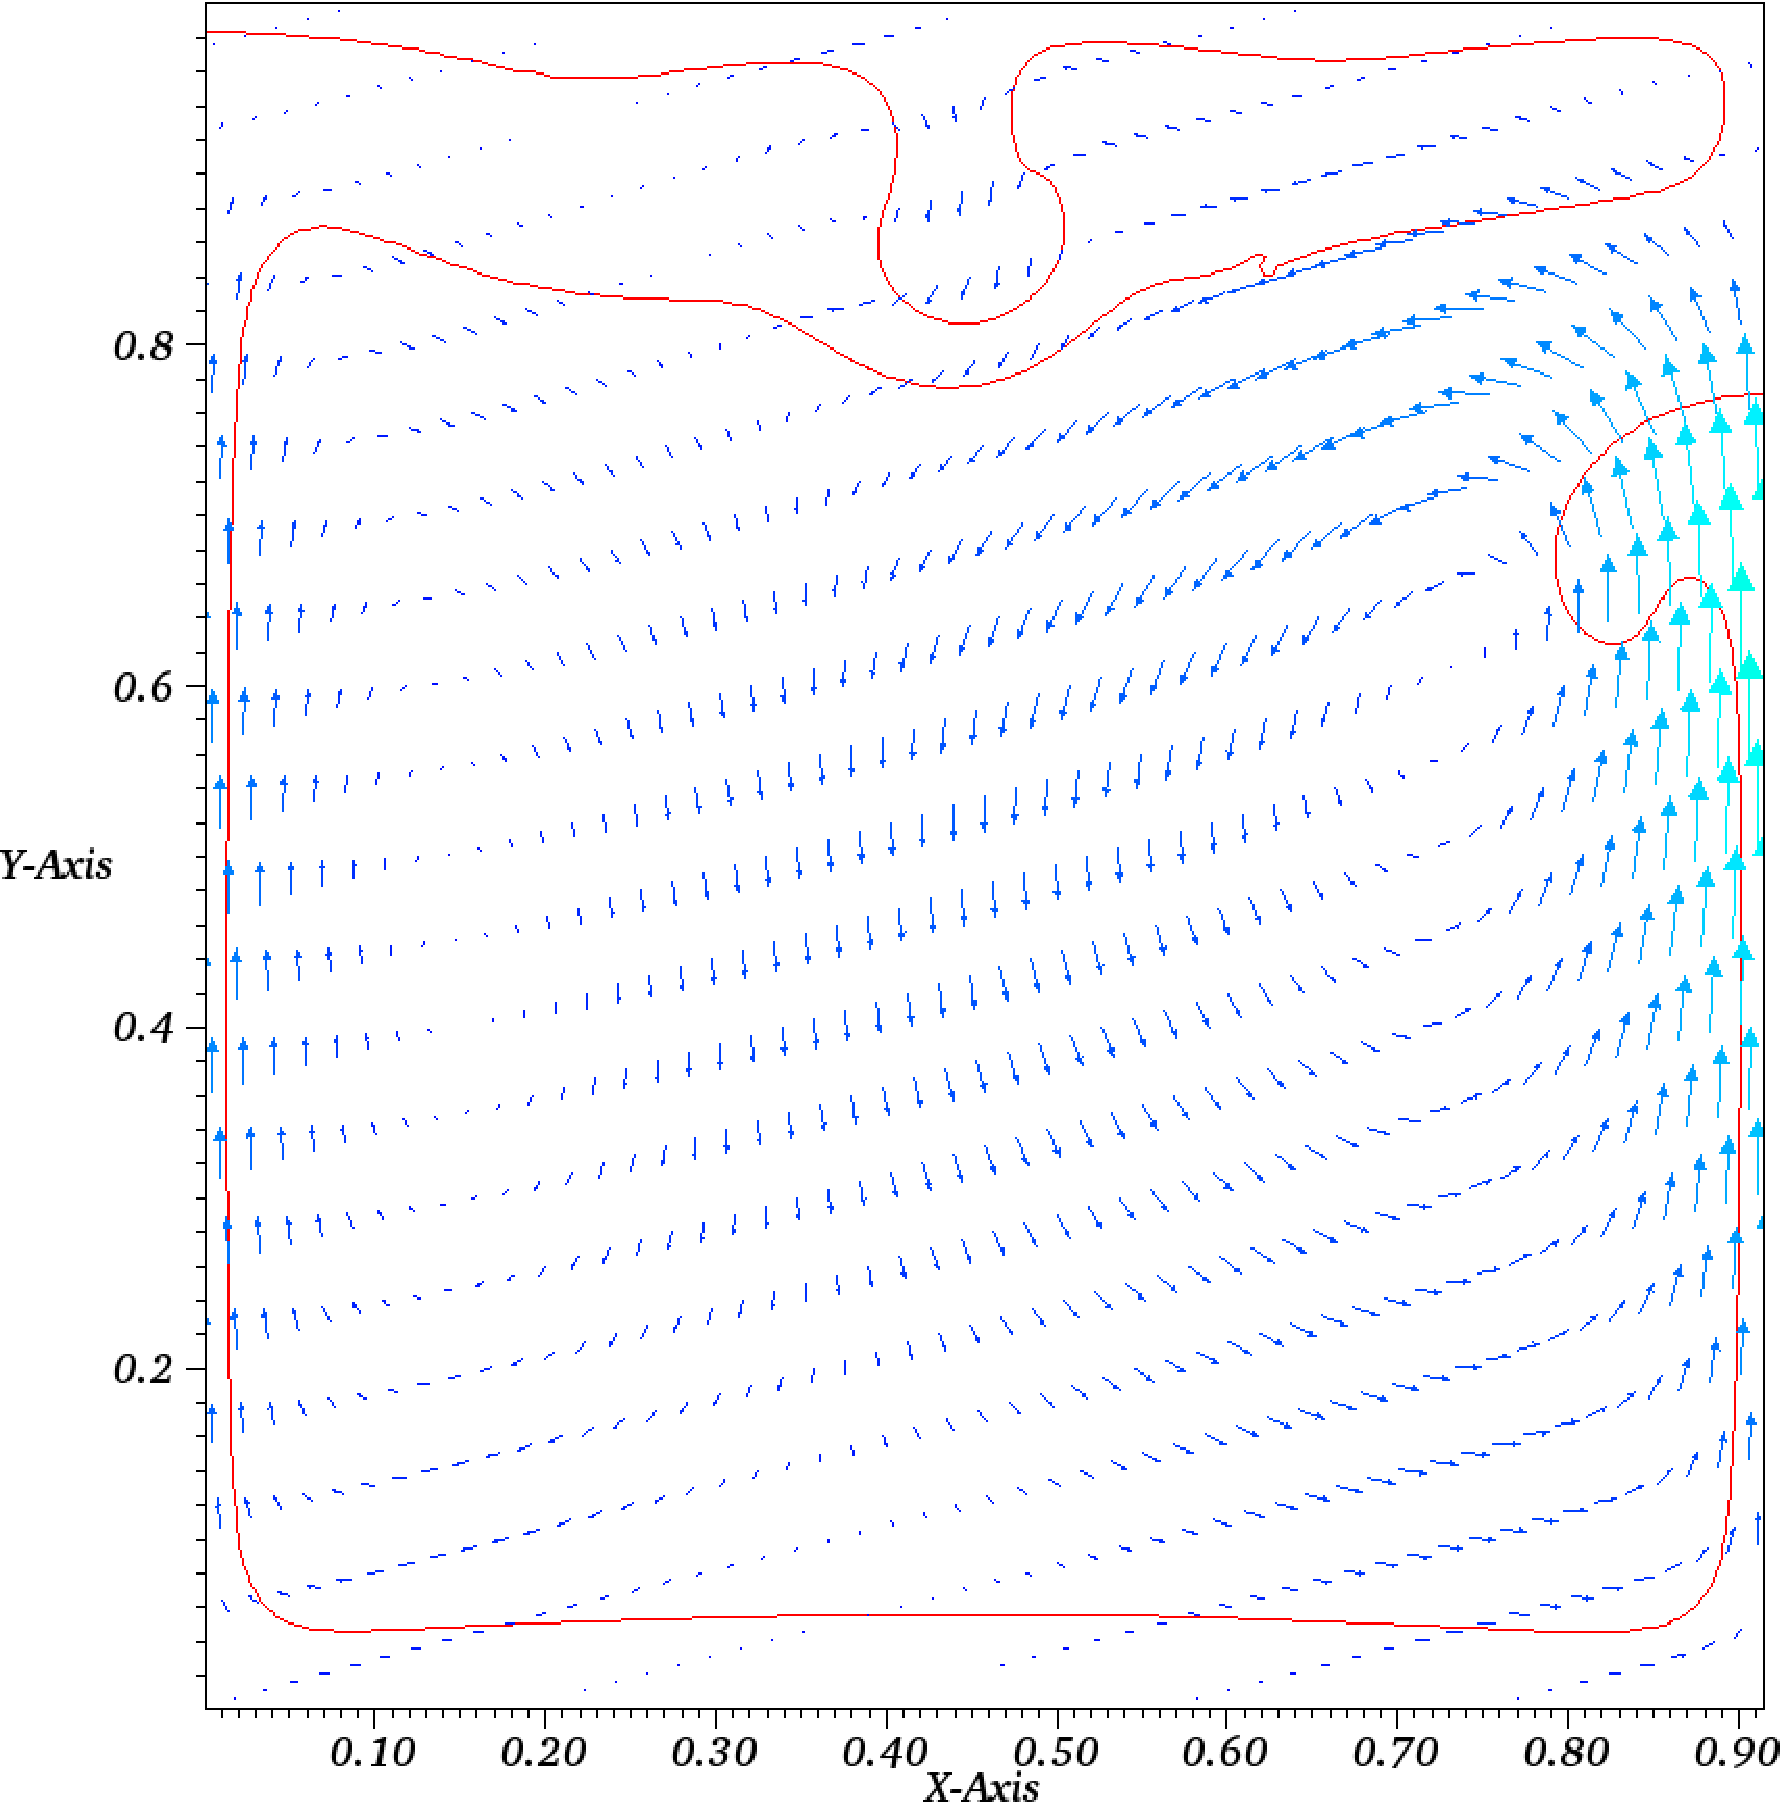
\includegraphics[scale=0.252]{RT2D200by200t1800}}
\caption{Simulation output of Rayleigh-Taylor instability.}
\label{RT2D OUTPUT2}
\end{figure}
%
%
%The Level Set Method can be applied to many areas of science, for example simulating subduction zones in geophysics, motion of bubbles, and flame propagation. Its also used in image processing. However, the Level Set Method does have limitations. The level set function can still become irregular after reinitialisation, leading to artifacts in the simulations, requiring more thought into the implementation of the reinitialisation step.
%
